\documentclass[12pt]{beamer}
\usepackage{Estilos/BeamerFC}
\usepackage{Estilos/ColoresLatex}
\usetheme{Warsaw}
\usecolortheme{seahorse}
%\useoutertheme{default}
\setbeamercovered{invisible}
% or whatever (possibly just delete it)
\setbeamertemplate{section in toc}[sections numbered]
\setbeamertemplate{subsection in toc}[subsections numbered]
\setbeamertemplate{subsection in toc}{\leavevmode\leftskip=3.2em\rlap{\hskip-2em\inserttocsectionnumber.\inserttocsubsectionnumber}\inserttocsubsection\par}
\setbeamercolor{section in toc}{fg=blue}
\setbeamercolor{subsection in toc}{fg=blue}
\setbeamercolor{frametitle}{fg=blue}
\setbeamertemplate{caption}[numbered]

\setbeamertemplate{footline}
\beamertemplatenavigationsymbolsempty
\setbeamertemplate{headline}{}


\makeatletter
\setbeamercolor{section in foot}{bg=gray!30, fg=black!90!orange}
\setbeamercolor{subsection in foot}{bg=blue!30}
\setbeamercolor{date in foot}{bg=black}
\setbeamertemplate{footline}
{
  \leavevmode%
  \hbox{%
  \begin{beamercolorbox}[wd=.333333\paperwidth,ht=2.25ex,dp=1ex,center]{section in foot}%
    \usebeamerfont{section in foot} \insertsection
  \end{beamercolorbox}%
  \begin{beamercolorbox}[wd=.333333\paperwidth,ht=2.25ex,dp=1ex,center]{subsection in foot}%
    \usebeamerfont{subsection in foot}  \insertsubsection
  \end{beamercolorbox}%
  \begin{beamercolorbox}[wd=.333333\paperwidth,ht=2.25ex,dp=1ex,right]{date in head/foot}%
    \usebeamerfont{date in head/foot} {T1 - Segunda presentación} \hspace*{2em}
    \insertframenumber{} / \inserttotalframenumber \hspace*{2ex} 
  \end{beamercolorbox}}%
  \vskip0pt%
}
\makeatother

\makeatletter
\patchcmd{\beamer@sectionintoc}{\vskip1.5em}{\vskip0.8em}{}{}
\makeatother
\usepackage{pifont}
\newcommand{\cmark}{\ding{51}}%
\newcommand{\xmark}{\ding{55}}%

\makeatletter
\setbeamertemplate{footline}
{
  \leavevmode%
  \hbox{%
  \begin{beamercolorbox}[wd=.333333\paperwidth,ht=2.25ex,dp=1ex,center]{section in foot}%
    \usebeamerfont{section in foot} \insertsection
  \end{beamercolorbox}%
  \begin{beamercolorbox}[wd=.333333\paperwidth,ht=2.25ex,dp=1ex,center]{subsection in foot}%
    \usebeamerfont{subsection in foot}  \insertsubsection
  \end{beamercolorbox}%
  \begin{beamercolorbox}[wd=.333333\paperwidth,ht=2.25ex,dp=1ex,right]{date in head/foot}%
    \usebeamerfont{date in head/foot} \insertshortdate{} \hspace*{2em}
    \insertframenumber{} / \inserttotalframenumber \hspace*{2ex} 
  \end{beamercolorbox}}%
  \vskip0pt%
}
\makeatother

\setbeamertemplate{navigation symbols}{}
\date{3 de abril}

\title{Sesión 5. Física}
\subtitle{Asesoría}

\begin{document}

\maketitle
\fontsize{14}{14}\selectfont
\spanishdecimal{.}

\section*{Contenido}
\frame[allowframebreaks]{\tableofcontents[currentsection, hideallsubsections]}


\section{Resolviendo el Ejercicio 2}
\frame{\tableofcontents[currentsection, hideothersubsections]}
\subsection{El problema a resolver}

\begin{frame}
\frametitle{Enunciado del Ejercicio 2}
En una persecución policial, el automóvil en fuga inicia con los siguientes desplazamientos:
\setbeamercolor{item projected}{bg=lava,fg=white}
\setbeamertemplate{enumerate items}{%
\usebeamercolor[bg]{item projected}%
\raisebox{1.5pt}{\colorbox{bg}{\color{fg}\footnotesize\insertenumlabel}}%
}
\begin{enumerate}[<+->]
\item $d_{1} = \SI{120}{\meter}, \theta = \ang{10}$
\item $d_{2} = \SI{900}{\meter}, \theta = \ang{100}$
\item $d_{3} = \SI{700}{\meter}, \theta = \ang{200}$
\item $d_{4} = \SI{500}{\meter}, \theta = \ang{300}$
\end{enumerate}
\end{frame}
\begin{frame}
\frametitle{Enunciado del Ejercicio 2}
Si una patrulla está en la posición donde inició el automóvil la fuga.
\\
\bigskip
\pause
¿Cuál es el desplazamiento que tiene que realizar la patrulla par encontrarse con el automóvil que se dio a la fuga?
\\
\bigskip
\pause
Determina el valor del desplazamiento resultante, con respecto al eje $x$ positivo.
\end{frame}
\begin{frame}
\frametitle{Método gráfico}
Nuevamente ocupamos el método gráfico para encontrar el vector resultante.
\\
\bigskip
\pause
A continuación se revisan los desplazamientos del automóvil en fuga.
\end{frame}
\begin{frame}[plain]
\begin{figure}
    \centering
    \begin{tikzpicture}[scale=0.8]
        % \draw[thin, gray!40] (-7, 0) grid (5, 9);
        \draw [-stealth, thick] (0, 0) -- (1.181, 0.208) node [above, near end] {$d_{1}$};
        \draw (0, 0) -- (1, 0);
        \draw (0.5, 0) arc(0:10:0.4);
        \node at (1.5, -0.3) {$\theta_{1} = \ang{10}$};
        \pause
        \draw [-stealth, thick] (1.181, 0.208) -- (-0.381, 9.071) node [right, midway] {$d_{2}$};
        \draw (1.181, 0.208) -- (2.181, 0.208);
        \draw (1.681, 0.208) arc(0:100:0.5);
        \node at (3.1, 0.5) {$\theta_{2} = \ang{100}$};
        \pause
        \draw [-stealth, thick] (-0.381, 9.071) -- (-6.958, 6.677) node [above, midway] {$d_{3}$};
        \draw (-0.381, 9.071) -- (0.6, 9.071);
        \draw (0.3, 9.071) arc(0:200:0.5);
        \node at (1.4, 9.5) {$\theta_{3} = \ang{200}$};
        \pause
        \draw [-stealth, thick] (-6.958, 6.677) -- (-2.655, 4.177) node [above, midway] {$d_{4}$};
        \draw (-6.958, 6.677) -- (-5.958, 6.677);
        \draw (-6.3, 6.677) arc(0:300:0.4);
        \node at (-6.5, 7.8) {$\theta_{4} = \ang{300}$};
        \pause
        \draw [-stealth, thick, color=blue] (0, 0) -- (-2.655, 4.177) node [below, midway] {$d_{R}$};
        \pause
        \draw [thick, color=blue] (0.4, 0) arc(0:130:0.38);
        \node at (-1, 0.3) [color=blue] {$\theta_{R}$};
    \end{tikzpicture}
\end{figure}
\end{frame}
\begin{frame}
\frametitle{Solución analítica}
Repetimos el procedimiento para obtener la solución analítica mediante la suma de las componentes de cada vector en las direcciones $x$ e $y$.
\end{frame}
\begin{frame}
\frametitle{Simplificando el problema}
Para resolver de manera más ágil el ejercicio, \pause a partir del ángulo del vector que se indica, identificamos el cuadrante al que pertenece.
\\
\bigskip
\pause
De esta manera tendremos las correspondientes expresiones para calcular las componentes de cada uno de ellos tanto en la dirección $x$ como en $y$.
\end{frame}
\begin{frame}
\frametitle{Componentes del vector $d_{1}$}
Como $\theta_{1} = \ang{10} < \ang{90}$
el vector $d_{1}$ se encuentra en el cuadrante I.
\\
\bigskip
\pause
Por lo tanto:
\pause
\begin{eqnarray*}
\begin{aligned}
d_{1x} &= \cos \theta_{1} \cdot d_{1} \pause = \cos \ang{10} \, \cdot \SI{120}{\meter} = \pause \SI{118.17}{\meter} \\[0.5em] \pause
d_{1y} &= \sin \theta_{1} \cdot d_{1} \pause =\sin \ang{10} \, \cdot \SI{120}{\meter} = \pause \SI{20.83}{\meter}
\end{aligned}
\end{eqnarray*}
\end{frame}
\begin{frame}
\frametitle{Componentes del vector $d_{2}$}
Para el vector $d_{2}$ revisamos que el ángulo:
\pause
\begin{eqnarray*}
\ang{90} < \theta_{2} = \ang{100} < \ang{180}
\end{eqnarray*}
\pause
por lo que el vector $d_{2}$ se encuentra en el cuadrante II.
\end{frame}
\begin{frame}
\frametitle{Componentes del vector $d_{2}$}
Tenemos que ocupar un ángulo auxiliar $\alpha$, que es el ángulo suplementario, es decir:
\pause
\begin{align*}
\theta = \ang{180} - \alpha
\end{align*}
\begin{minipage}{0.6\linewidth}
Por tanto:
\begin{eqnarray*}
\alpha = \ang{180} - \ang{100} = \pause \ang{80}
\end{eqnarray*}
\end{minipage}
\begin{minipage}{0.35\linewidth}
\begin{figure}
\centering
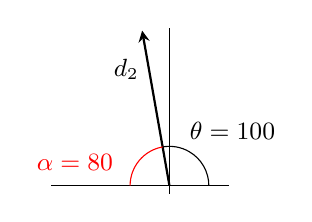
\begin{tikzpicture}
  \draw (-1.5, 0) -- (0.75, 0);
  \draw (0, -0.1) -- (0, 2);
  \draw [-stealth, thick] (0, 0) -- (-0.347, 1.969) node [left, near end] {\small{$d_{2}$}};
  \draw (0.5, 0) arc(0:100:0.5);
  \node at (0.8, 0.7) {\small{$\theta = \ang{100}$}};
  \draw [color=red] (-0.5, 0) arc(180:100:0.5);
  \node at (-1.2, 0.3) [color=red] {\small{$\alpha = \ang{80}$}};
\end{tikzpicture}
\end{figure}
\end{minipage}
\end{frame}
\begin{frame}
\frametitle{Componentes del vector $d_{2}$}
\begin{figure}
\centering
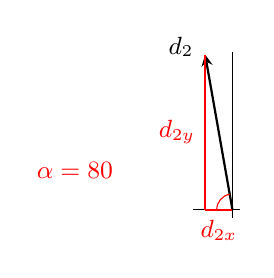
\begin{tikzpicture}
  \draw (-0.5, 0) -- (0.1, 0);
  \draw (0, -0.1) -- (0, 2);
  \draw [-stealth, thick] (0, 0) -- (-0.347, 1.969) node [left, pos=1.05] {\small{$d_{2}$}};
  \draw [color=red] (-0.2, 0) arc(180:100:0.2);
  \node at (-2, 0.5) [color=red] {\small{$\alpha = \ang{80}$}};
  \draw [thick, color=red] (0, 0) -- (-0.347, 0) node [below, midway] {\small{$d_{2x}$}};
  \draw [thick, color=red] (-0.347, 0) -- (-0.347, 1.969) node [left, midway] {\small{$d_{2y}$}};
\end{tikzpicture}
\end{figure}
Entonces las componentes del vector $d_{2}$ son:
\pause
\begin{eqnarray*}
\begin{aligned}
d_{2x} &= -\cos \alpha \cdot d_{2} \pause = -\cos \ang{80} \, \cdot \SI{900}{\meter} = \pause -\SI{156.28}{\meter} \\[0.5em] \pause
d_{2y} &= \sin \alpha \cdot d_{2} \pause = \sin \ang{80} \, \cdot \SI{900}{\meter} = \pause \SI{886.32}{\meter}
\end{aligned}
\end{eqnarray*}
\end{frame}
\begin{frame}
\frametitle{Componentes del vector $d_{3}$}
Para el vector $d_{3}$ vemos que el ángulo:
\pause
\begin{eqnarray*}
\ang{180} < \theta_{3} = \ang{200} < \ang{270}
\end{eqnarray*}
\pause
por lo que el vector $d_{3}$ se encuentra en el cuadrante III.
\end{frame}
\begin{frame}
\frametitle{Componentes del vector $d_{3}$}
Nuevamente tenemos que ocupar un ángulo auxiliar $\beta$, que es el ángulo complementario en el cuadrante III, es decir:
\pause
\begin{align*}
\theta = \ang{270} - \beta
\end{align*}
\end{frame}
\begin{frame}
\frametitle{Componentes del vector $d_{3}$}
\begin{eqnarray*}
\beta = \ang{270} - \ang{200} = \pause \ang{70}
\end{eqnarray*}
\pause
\vspace*{-1cm}
\begin{figure}
\centering
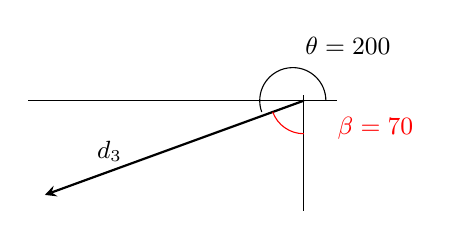
\begin{tikzpicture}[scale=0.7]
  \draw (-5, 0) -- (0.6, 0);
  \draw (0, 0.1) -- (0, -2);
  \draw [-stealth, thick] (0, 0) -- (-4.698, -1.71) node [above, near end] {\small{$d_{3}$}};
  \draw (0.4, 0) arc(0:200:0.6);
  \node at (0.8, 1) {\small{$\theta = \ang{200}$}};
  \draw [color=red] (0, -0.6) arc(270:200:0.6);
  \node at (1.3, -0.5) [color=red] {\small{$\beta = \ang{70}$}};
\end{tikzpicture}
\end{figure}
\end{frame}
\begin{frame}
\frametitle{Componentes del vector $d_{3}$}
\begin{figure}
  \centering
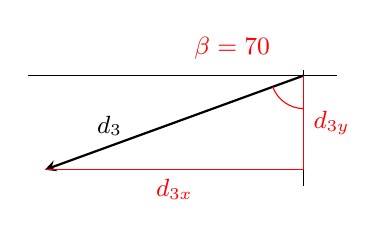
\begin{tikzpicture}[scale=0.7]
  \draw (-5, 0) -- (0.6, 0);
  \draw (0, 0.1) -- (0, -2);
  \draw [-stealth, thick] (0, 0) -- (-4.698, -1.71) node [above, near end] {\small{$d_{3}$}};
  
  \draw [color=red] (0, -0.6) arc(270:200:0.6);
  \node at (-1.3, 0.5) [color=red] {\small{$\beta = \ang{70}$}};
  \draw [color=red] (0, -1.71) -- (-4.698, -1.71) node [below, midway] {\small{$d_{3x}$}};
  \draw [color=red] (0, 0) -- (0, -1.71) node [right, midway] {\small{$d_{3y}$}};
\end{tikzpicture}
\end{figure}
Entonces las componentes del vector $d_{3}$ son:
\pause
\begin{eqnarray*}
\begin{aligned}
d_{3x} &= -\sin \beta \cdot d_{3} \pause = -\sin \ang{70} \, \cdot \SI{700}{\meter} = \pause -\SI{657.78}{\meter} \\[0.5em] \pause
d_{3y} &= -\cos \beta \cdot d_{3} \pause = -\cos \ang{70} \, \cdot \SI{700}{\meter} = \pause -\SI{239.41}{\meter}
\end{aligned}
\end{eqnarray*}
\end{frame}
\begin{frame}
\frametitle{Componentes del vector $d_{4}$}
Para el último vector $d_{4}$ vemos que el ángulo:
\pause
\begin{eqnarray*}
\ang{270} < \theta_{4} = \ang{300} < \ang{360}
\end{eqnarray*}
\pause
por lo que el vector $d_{4}$ se encuentra en el cuadrante IV.
\end{frame}
\begin{frame}
\frametitle{Componentes del vector $d_{4}$}
Nuevamente tenemos que ocupar un ángulo auxiliar $\psi$, que es el ángulo suplementario en el cuadrante IV.
\pause
\begin{align*}
\theta = \ang{360} - \psi
\end{align*}
\end{frame}
\begin{frame}
\frametitle{Componentes del vector $d_{4}$}
Siendo entonces:
\pause
\begin{eqnarray*}
\psi = \ang{360} - \ang{300} = \pause \ang{60}
\end{eqnarray*}
\vspace*{-1cm}
\begin{figure}
\centering
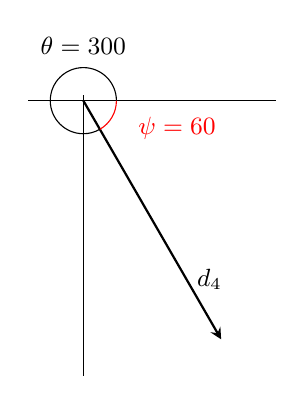
\begin{tikzpicture}[scale=0.7]
  \draw (-1, 0) -- (3.5, 0);
  \draw (0, 0.1) -- (0, -5);
  \draw [-stealth, thick] (0, 0) -- (2.5, -4.33) node [right, near end] {\small{$d_{4}$}};
  \draw (0.6, 0) arc(0:300:0.6);
  \node at (0, 1) {\small{$\theta = \ang{300}$}};
  \draw [color=red] (0.6, 0) arc(360:300:0.6);
  \node at (1.7, -0.5) [color=red] {\small{$\psi = \ang{60}$}};
\end{tikzpicture}
\end{figure}
\end{frame}
\begin{frame}
\frametitle{Componentes del vector $d_{4}$}
\begin{figure}
  \centering
  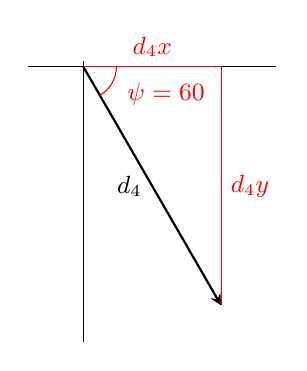
\begin{tikzpicture}[scale=0.7]
  \draw (-1, 0) -- (3.5, 0);
  \draw (0, 0.1) -- (0, -5);
  \draw [-stealth, thick] (0, 0) -- (2.5, -4.33) node [left, midway] {\small{$d_{4}$}};
  \draw [color=red] (0.6, 0) arc(360:300:0.6);
  \node at (1.5, -0.5) [color=red] {\small{$\psi = \ang{60}$}};
  \draw [color=red] (0, 0) -- (2.5, 0) node [above, midway] {\small{$d_4x$}};
  \draw [color=red] (2.5, 0) -- (2.5, -4.33) node [right, midway] {\small{$d_4y$}};
\end{tikzpicture}
\end{figure}
Entonces las componentes del vector $d_{4}$ son:
\pause
\begin{eqnarray*}
\begin{aligned}
d_{4x} &= \cos \psi \cdot d_{4} \pause = \cos \ang{60} \, \cdot \SI{500}{\meter} = \pause \SI{250}{\meter} \\[0.5em] \pause
d_{4y} &= -\sin \psi \cdot d_{4} \pause = - \sin \ang{60} \, \cdot \SI{500}{\meter} = \pause = -\SI{433.01}{\meter}
\end{aligned}
\end{eqnarray*}
\end{frame}
\begin{frame}
\frametitle{Sumando las componentes}
Una vez que ya hemos calculado las componentes en de los vectores en las direcciones $x$, $y$, ahora pasamos a sumar el valor de cada una de ellas para obtener las componentes del vector resultante.
\end{frame}
\begin{frame}
\frametitle{Componentes del vector resultante}
Para la componente $d_{Rx}$ se tiene entonces que:
\pause
\begin{eqnarray*}
\begin{aligned}
d_{Rx} &= \nsum_{n=1}^{4} d_{ix} = \pause d_{1x} + d_{2x} + d_{3x} + d_{4x} = \\[0.5em] \pause
&= \SI{118.17}{\meter} {+} (-\SI{156.28}{\meter}) {+} (-\SI{657.78}{\meter}) {+} \SI{250}{\meter} = \\[0.5em] \pause
&= -\SI{445.89}{\meter}
\end{aligned}
\end{eqnarray*}
\end{frame}
\begin{frame}
\frametitle{Componentes del vector resultante}
Ahora para la componente $d_{Ry}$ se tiene que:
\pause
\begin{eqnarray*}
\begin{aligned}
d_{Ry} &= \nsum_{n=1}^{4} d_{iy} = \pause d_{1y} + d_{2y} + d_{3y} + d_{4y} = \\[0.5em] \pause
&= \SI{20.83}{\meter} {+} \SI{886.32}{\meter} {+} (-\SI{239.41}{\meter}) {+} (-\SI{433.01}{\meter}) = \\[0.5em] \pause
&= \SI{234.73}{\meter}
\end{aligned}
\end{eqnarray*}
\end{frame}
\begin{frame}
\frametitle{Magnitud del vector resultante}
Una vez obtenidas las componentes del vector resultante, podemos obtener su magnitud:
\pause
\begin{eqnarray*}
\begin{aligned}
\abs{d_{R}} &= \sqrt{ (d_{Rx})^{2} + (d_{Ry})^{2} } = \\[0.5em] \pause
&= \sqrt{(-\SI{445.89}{\meter})^{2} + (\SI{234.73}{\meter})^{2}} = \\[0.5em] \pause
&= \sqrt{ \SI{198817.89}{\square\meter} + \SI{55098.17}{\square\meter} } = \\[0.5em] \pause
&= \sqrt{\SI{253916.06}{\square\meter}} = \\[0.5em] \pause
&= \SI{503.90}{\meter}
\end{aligned}
\end{eqnarray*}
\end{frame}
\begin{frame}
\frametitle{El ángulo del vector resultante}
De los valores de las componentes $d_{Rx}$, $d_{Ry}$ podemos reconocer el vector resultante se encuentra en el cuadrante II:
\\
\pause
\begin{minipage}{0.4\linewidth}
\begin{align*}
d_{Rx} &= -\SI{445.89}{\meter} \\[0.5em]
d_{Ry} &=  \SI{234.73}{\meter}
\end{align*}
\end{minipage}
\hspace{1cm}
\begin{minipage}{0.35\linewidth}
\begin{figure}
  \centering
  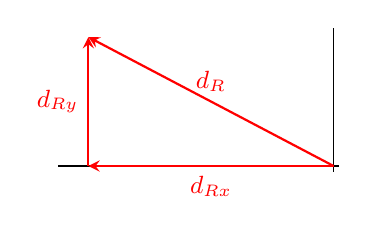
\begin{tikzpicture}[scale=0.7]
  \draw (-5, 0) -- (0.1, 0);
  \draw (0, -0.1) -- (0, 2.5);
  \draw [-stealth, thick, color=red] (0, 0) -- (-4.45, 0) node [below, midway] {\small{$d_{Rx}$}};
  \draw [-stealth, thick, color=red] (-4.45, 0) -- (-4.45, 2.34) node [left, midway] {\small{$d_{Ry}$}};
  \draw [-stealth, thick, color=red] (0, 0) -- (-4.45, 2.34) node [above, midway] {\small{$d_{R}$}};
  \end{tikzpicture}
  \end{figure}
\end{minipage}
\end{frame}
\begin{frame}
\frametitle{El ángulo del vector resultante}
\begin{minipage}{0.35\linewidth}
\begin{figure}
\centering
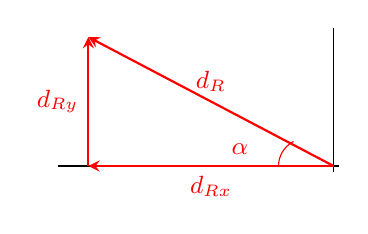
\begin{tikzpicture}[scale=0.7]
  \draw (-5, 0) -- (0.1, 0);
  \draw (0, -0.1) -- (0, 2.5);
  \draw [-stealth, thick, color=red] (0, 0) -- (-4.45, 0) node [below, midway] {\small{$d_{Rx}$}};
  \draw [-stealth, thick, color=red] (-4.45, 0) -- (-4.45, 2.34) node [left, midway] {\small{$d_{Ry}$}};
  \draw [-stealth, thick, color=red] (0, 0) -- (-4.45, 2.34) node [above, midway] {\small{$d_{R}$}};
  \draw [color=red] (-1, 0) arc(180:117:0.5);
  \node at (-1.7, 0.3) [color=red] {\small{$\alpha$}};
\end{tikzpicture}
\end{figure}
\end{minipage}
\hspace{0.25cm}
\begin{minipage}{0.6\linewidth}
Ocuparemos un ángulo auxiliar $\alpha$, de tal manera que:
\begin{eqnarray*}
\begin{aligned}
\tan \alpha &= - \dfrac{d_{Ry}}{d_{Rx}} = \\[0.5em] \pause
\tan \alpha &= - \dfrac{\SI{234.73}{\meter}}{\SI{445.89}{\meter}} = \\[0.5em] \pause
\tan \alpha &= - 0.5264
\end{aligned}
\end{eqnarray*}
\end{minipage}
\end{frame}
\begin{frame}
\frametitle{El ángulo del vector resultante}
Pero como queremos el valor del ángulo, ocupamos la función inversa, el arco tangente:
\pause
\begin{eqnarray*}
\begin{aligned}
\arctan(\tan \alpha) &= \arctan(-0.5264) = \\[0.5em] \pause
\alpha &= -\ang{27.63}
\end{aligned}
\end{eqnarray*}
\pause
El signo negativo nos indica que se está midiendo desde el eje $x$ negativo, en el sentido horario del reloj.
\end{frame}
\begin{frame}
\frametitle{El ángulo del vector resultante}
Como sabemos que $\alpha$ es ángulo suplementario, entonces ocupamos su valor positivo:
\pause
\begin{minipage}{0.5\linewidth}
\begin{eqnarray*}
\begin{aligned}
\theta_{R} &= \ang{180} - \alpha = \\[0.5em] \pause
&= \ang{180} - \ang{27.63} = \\[0.5em] \pause
\theta_{R} &= \ang{152.37}
\end{aligned}
\end{eqnarray*}
\end{minipage}
\begin{minipage}{0.35\linewidth}
\begin{figure}
\centering
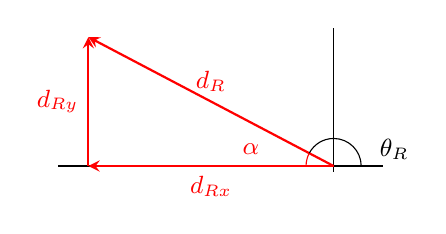
\begin{tikzpicture}[scale=0.7]
  \draw (-5, 0) -- (0.9, 0);
  \draw (0, -0.1) -- (0, 2.5);
  \draw [-stealth, thick, color=red] (0, 0) -- (-4.45, 0) node [below, midway] {\small{$d_{Rx}$}};
  \draw [-stealth, thick, color=red] (-4.45, 0) -- (-4.45, 2.34) node [left, midway] {\small{$d_{Ry}$}};
  \draw [-stealth, thick, color=red] (0, 0) -- (-4.45, 2.34) node [above, midway] {\small{$d_{R}$}};
  \draw [color=red] (-0.5, 0) arc(180:152:0.5);
  \node at (-1.5, 0.3) [color=red] {\small{$\alpha$}};
  \draw (0.5, 0) arc(0:152:0.5);
  \node at (1.1, 0.3) {\small{$\theta_{R}$}};
\end{tikzpicture}
\end{figure}
\end{minipage}
\end{frame}
\begin{frame}
\frametitle{Respuesta al ejercicio}
Entonces se tiene como respuesta que el vector resultante tiene como magnitud y el ángulo de dirección con respecto al eje $x$ horizontal:
\begin{align*}
\text{Magnitud} &= \SI{503.90}{\meter} \\[0.5em]
\text{Ángulo} &= \ang{152.37}
\end{align*}
\end{frame}

\section{Sobre el ángulo}
\frame{\tableofcontents[currentsection, hideothersubsections]}
\subsection{Revisando la referencia}

\begin{frame}
\frametitle{La referencia para el ángulo}
Es muy importante revisar la referencia en la que se indica el ángulo ya sea para cada vector o para el vector resultante.
\\
\bigskip
\pause
En los ejercicios anteriores hemos tenido: \emph{... cuál es el valor del ángulo del desplazamiento resultante, medido respecto al eje $x$ positivo.}
\end{frame}
\begin{frame}
\frametitle{Con respecto al eje $x$ positivo}
Si el enunciado indica que debemos de tomar como referencia el eje $x$ positivo, entonces para cada vector en el sistema a resolver, el ángulo debe de medirse con respecto a este eje.
\end{frame}
\begin{frame}
\frametitle{El caso de los cuadrantes}
En los cuadrantes II y III vimos que por la trigonometría involucrada, hay un cambio con respecto a las funciones trigonométricas para obtener las componentes de los vectores en los ejes $x$ e $y$.
\end{frame}
\begin{frame}
\frametitle{Cuando no se indica la referencia}
Es posible que el enunciado de un ejercicio no nos indique la referencia con respecto al eje $x$ para medir el ángulo.
\\
\bigskip
\pause
En estos casos debemos de apoyarnos con la geometría en el plano cartesiano.
\end{frame}
\begin{frame}
\frametitle{Ejemplo 1}
Veamos el siguiente ejemplo donde nos piden calcular las componentes del vector con el ángulo $\theta$ que se indica:
\pause
\begin{figure}
\centering
\begin{tikzpicture}[scale=0.8]
    \draw (-2, 0) -- (2, 0);
    \draw (0, -1) -- (0, 5) ;
    \draw [-stealth, thick] (0, 0) -- (-1.368, 3.758) node [left, near end] {$\va{a}$};
    \draw (0, 0.75) arc(90:110:0.8);
    \node at (1.5, 0.75) {$\theta = \ang{20}$};
\end{tikzpicture}
\end{figure}
\end{frame}
\begin{frame}
\frametitle{Revisando el caso en el cuadrante II}
\begin{minipage}{0.35\linewidth}
\begin{figure}
  \centering
  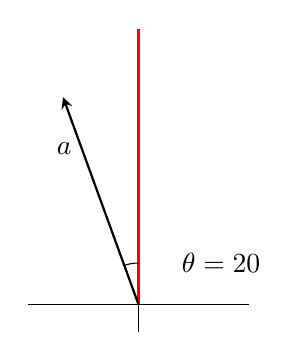
\begin{tikzpicture}[scale=0.7]
      \draw (-2, 0) -- (2, 0);
      \draw [thick, color=red] (0, 0) -- (0, 5) ;
      \draw (0, 0) -- (0, -0.5) ;
      \draw [-stealth, thick] (0, 0) -- (-1.368, 3.758) node [left, near end] {$\va{a}$};
      \draw (0, 0.75) arc(90:110:0.8);
      \node at (1.5, 0.75) {$\theta = \ang{20}$};
  \end{tikzpicture}
  \end{figure}
\end{minipage}
\begin{minipage}{0.6\linewidth}
De la figura reconocemos que el ángulo $\theta$ se mide a partir del eje $y$ positivo. \pause Si lo medimos desde el eje $x$ positivo, el ángulo sería $\theta = \ang{90} + \ang{20} = \ang{110}$
\end{minipage}
\end{frame}
\begin{frame}
\frametitle{El ángulo complementario}
Para obtener las componentes del vector $\va{a}$ se requiere tomar el ángulo complementario $\alpha$ en el segundo cuadrante.
\end{frame}
\begin{frame}
\frametitle{El ángulo complementario}
\begin{minipage}{0.35\linewidth}
\begin{figure}
  \centering
  \begin{tikzpicture}[scale=0.7]
      \draw (-2, 0) -- (2, 0);
      \draw (0, -1) -- (0, 5) ;
      \draw [-stealth, thick] (0, 0) -- (-1.368, 3.758) node [left, near end] {$\va{a}$};
      \draw (0, 0.75) arc(90:110:0.8);
      \node at (1.5, 0.75) {$\theta = \ang{20}$};
      \draw [thick, color=red] (-0.75, 0) arc(180:110:0.8);
      \node at (-1.2, 0.5) {$\alpha$};
  \end{tikzpicture}
  \end{figure}
\end{minipage}
\begin{minipage}{0.6\linewidth}
Se tiene entonces que:
\pause
\begin{align*}
\alpha &= \ang{90} - \theta = \ang{90} - \ang{20} = \\[0.5em]
\alpha &= \ang{70}
\end{align*}
\end{minipage}  
\end{frame}
\begin{frame}
\frametitle{Las componentes}
\begin{minipage}{0.35\linewidth}
\begin{figure}
\centering
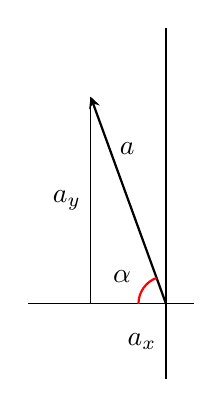
\begin{tikzpicture}[scale=0.7]
    \draw (-2.5, 0) -- (0.5, 0);
    \draw (0, -1) -- (0, 5) ;
    \draw [-stealth, thick] (0, 0) -- (-1.368, 3.758) node [right, near end] {$\va{a}$};
    \draw [thick, color=red] (-0.5, 0) arc(180:110:0.5);
    \node at (-0.8, 0.5) {$\alpha$};
    \draw (-1.368, 0) -- (-1.368, 3.758) node [left, midway] {$a_{y}$};
    \draw (0, 0) -- (0, -1.368) node [left, midway] {$a_{x}$};
\end{tikzpicture}
\end{figure}
\end{minipage}
\begin{minipage}{0.6\linewidth}
Por lo que ya podemos calcular las componentes $a_{x}$ y $a_{y}$:
\pause
\begin{align*}
a_{x} &= - \cos \alpha \cdot \abs{a} \\[0.5em] 
a_{y} &= \sin \alpha \cdot \abs{a}
\end{align*}
\end{minipage}
\end{frame}
\begin{frame}
\frametitle{Ejemplo 2}
Veamos el siguiente ejemplo donde nos piden calcular las componentes del vector con el ángulo $\theta$ que se indica:
\pause
\begin{figure}
\centering
\begin{tikzpicture}[scale=0.8]
    \draw (-2, 0) -- (0.5, 0);
    \draw (0, 0.5) -- (0, -4) ;
    \draw [-stealth, thick] (0, 0) -- (-2, -3.464) node [above, near end] {$\va{b}$};
    \draw (0, -0.5) arc(270:240:0.5);
    \node at (1.3, -0.5) {$\theta = \ang{30}$};
\end{tikzpicture}
\end{figure}
\end{frame}
\begin{frame}
\frametitle{Ocupando un eje como referencia}
\begin{minipage}{0.35\linewidth}
\begin{figure}
\centering
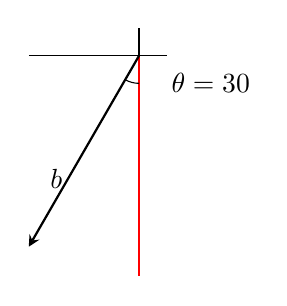
\begin{tikzpicture}[scale=0.7]
    \draw (-2, 0) -- (0.5, 0);
    \draw [thick, color=red] (0, 0) -- (0, -4);
    \draw (0, 0) -- (0, 0.5);
    \draw [-stealth, thick] (0, 0) -- (-2, -3.464) node [above, near end] {$\va{b}$};
    \draw (0, -0.5) arc(270:240:0.5);
    \node at (1.3, -0.5) {$\theta = \ang{30}$};
\end{tikzpicture}
\end{figure}
\end{minipage}
\begin{minipage}{0.6\linewidth}
Tenemos un ángulo $\theta = \ang{30}$ con respecto al eje $y$ negativo.
\\
Podemos ocupar como referencia el eje $x$ negativo, usando para ello, el ángulo complementario en este III cuadrante.
\end{minipage}
\end{frame}
\begin{frame}
\frametitle{Ocupando un eje como referencia}
\begin{minipage}{0.35\linewidth}
\begin{figure}
\centering
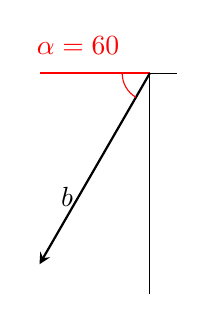
\begin{tikzpicture}[scale=0.7]
    \draw [thick, color=red] (-2, 0) -- (0, 0);
    \draw (0, 0) -- (0.5, 0);
    \draw (0, 0) -- (0, -4);
    \draw [-stealth, thick] (0, 0) -- (-2, -3.464) node [above, near end] {$\va{b}$};
    \draw [color=red] (-0.5, 0) arc(180:240:0.5);
    \node at (-1.3, 0.5) [color=red] {$\alpha = \ang{60}$};
\end{tikzpicture}
\end{figure}
\end{minipage}
\begin{minipage}{0.6\linewidth}
Tenemos un ángulo $\alpha = \ang{60}$ con respecto al eje $x$ negativo.
\end{minipage}
\end{frame}
\begin{frame}
\frametitle{Los valores de las componentes}
Veremos que se obtienen los mismo valores de las componentes del vector al utilizar cualquiera de los dos ángulos $\theta$ o $\alpha$.
\\
\bigskip
\pause
Si consideramos que la magnitud del vector $\va{b}$ es $\abs{\va{b}} = 3$.
\end{frame}
\begin{frame}
\frametitle{Los valores de las componentes}
\begin{minipage}{0.35\linewidth}
\begin{figure}
\centering
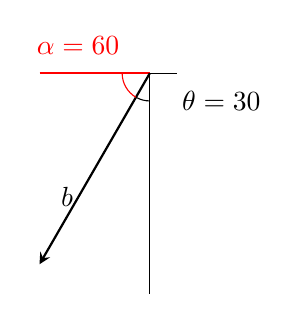
\begin{tikzpicture}[scale=0.7]
    \draw [thick, color=red] (-2, 0) -- (0, 0);
    \draw (0, 0) -- (0.5, 0);
    \draw (0, 0) -- (0, -4);
    \draw [-stealth, thick] (0, 0) -- (-2, -3.464) node [above, near end] {$\va{b}$};
    \draw (0, -0.5) arc(270:240:0.5);
    \node at (1.3, -0.5) {$\theta = \ang{30}$};
    \draw [color=red] (-0.5, 0) arc(180:240:0.5);
    \node at (-1.3, 0.5) [color=red] {$\alpha = \ang{60}$};
\end{tikzpicture}
\end{figure}
\end{minipage}
\begin{minipage}{0.6\linewidth}
La componente $b_{x}$ es:
\pause
\begin{eqnarray*}
\begin{aligned}
b_{x} &= - \sin \theta \cdot \abs{\va{b}} = \pause -(\sin \ang{30})(3) = \\[0.5em] \pause
&= -(0.5)(3) = \pause -1.5 \\[0.5em] \pause
b_{x} &= -\sin \alpha \cdot \abs{\va{b}} = \pause - (\cos \ang{60})(3) = \\[0.5em] \pause
&= - (0.5)(3) = \pause - 1.5
\end{aligned}
\end{eqnarray*}
\end{minipage}
\end{frame}
\begin{frame}
\frametitle{Los valores de las componentes}
\begin{minipage}{0.35\linewidth}
  \begin{figure}
\centering
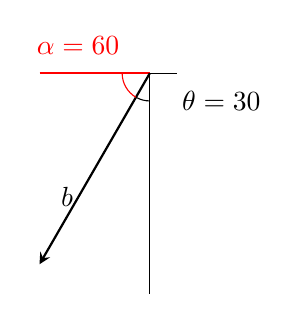
\begin{tikzpicture}[scale=0.7]
    \draw [thick, color=red] (-2, 0) -- (0, 0);
    \draw (0, 0) -- (0.5, 0);
    \draw (0, 0) -- (0, -4);
    \draw [-stealth, thick] (0, 0) -- (-2, -3.464) node [above, near end] {$\va{b}$};
    \draw (0, -0.5) arc(270:240:0.5);
    \node at (1.3, -0.5) {$\theta = \ang{30}$};
    \draw [color=red] (-0.5, 0) arc(180:240:0.5);
    \node at (-1.3, 0.5) [color=red] {$\alpha = \ang{60}$};
\end{tikzpicture}
\end{figure}
\end{minipage}
\begin{minipage}{0.6\linewidth}
La componente $b_{y}$ es:
\begin{eqnarray*}
\begin{aligned}
b_{y} &= - \cos \theta \cdot \abs{\va{b}} = \pause - (\cos \ang{30})(3) = \\[0.5em] \pause
&= - (0.866)(3) = \pause - 2.59 \\[0.5em] \pause
b_{y} &= - \sin \alpha \cdot \abs{\va{b}} = \pause - (\sin \ang{60})(3) = \\[0.5em] \pause
&= - (0.866)(3) = \pause - 2.59
\end{aligned}
\end{eqnarray*}
\end{minipage}
\end{frame}
\begin{frame}
\frametitle{Recomendación para el ángulo}
Como hemos revisado, se obtiene el valor de la componente del vector, ya sea utilizando el ángulo que se nos indica en el enunciado, o su complemento.
\end{frame}
\begin{frame}
\frametitle{Recomendación para el ángulo}
Se recomienda utilizar el ángulo que nos permita calcular la componente del vector en el eje $x$ en cada cuadrante, de tal manera que se ocupa la función trigonométrica \textbf{coseno}, \pause mientras que para la componente en $y$, sea la función \textbf{seno}.
\end{frame}

\end{document}